In this section, we first present experimental simulation results and
then validate the mathematical model presented in Section~\ref{model}.

\subsection{Experimental Setup}
In order to quantify the impact of our energy conservation methods,
we use various workloads that approximate usage in a cloud storage
system. The three workloads come from Google, the University of
Connecticut Hornet HPC system, and the GRID5000 platform. These workloads
are described in more detail below. The jobs in these workloads
are tied to users and each job is assumed to use the storage system equally.

\subsubsection{Workloads}
\paragraph{Google Trace}
The Google Trace is a log of jobs that are run in Google's cloud
system~\cite{clusterdata:Wilkes2011}. This trace has 29 days of data
collected from nearly 11,000 machines in May 2011 and it stores
detailed information (including storage space used) for each \textit{task},
\textit{job} and \textit{machine event}. We use the data from individual tasks in the
evaluations as each job comprises multiple tasks. Each task has a status
code indicating the current status of the task - such as submission, failure,
re-submission, completion etc. For our test purposes, we only consider tasks
that are submitted and completed successfully. The Google trace is a highly 
intensive workload, consisting of nearly 16 million tasks. We found the number
of users in this workload to be 100 (after unhashing the user names).

\paragraph{Hornet Cluster}
The Hornet Cluster~\cite{hornet} is a high end cluster at the University
of Connecticut consisting of 64 nodes where each node has 12 Intel Xeon X5650
Westmere cores, 48 GB of RAM and 500 GB of storage. Information about each
job executed on this cluster is recorded in the log files. For each job, the log files
provide the identifier of the user who submitted the job, in addition to the
submission and completion times. The log file comprises 25 months of data
collected between September 2011 and October 2013. While the Hornet cluster
is not a cloud system, it is representative of cluster jobs that may run on
a cloud compute system. The Hornet cluster workload includes about 145,000
jobs from 307 users.

\paragraph{GRID5000 Workload}
GRID5000 is a grid platform located in France comprising of nine separate computing
sites with a total of fifteen clusters available. Although a grid may not necessarily
be classified as a cloud platform, it has an architecture similar to a cloud system,
making GRID5000 a useful workload for our evaluations. GRID5000 workload~\cite{grid5000}
stores information about jobs submitted between May 2004 and November 2006. There is
no record of storage space usage in this workload.  Therefore, we randomly generated
that for each user. GRID5000 workload consists of nearly one million jobs from 645
users. 

\subsubsection{Test Parameters}
We test each workload with the parameters shown in Table~\ref{tbl:params}. We assume each storage
node consumes 300 Watts of power~\cite{DBLP:journals/computer/BianchiniR04}.

\begin{table}[!htbp]
 \begin{center}
  \begin{tabular}{|l|l|} \hline
Test Parameter & Values \\ \hline
Total number of nodes          & 64 \\ \hline
Number of nodes allocated        & 8 \\
for each user              & \\ \hline
Allocation methods           & Fixed, Dynamic Greedy, Correlation-Based \\ \hline
Low-energy mode             & Turn Off \\ \hline
Inactivity threshold          & 300, 1800, 3600 s \\ \hline
Startup time              & 30, 60, 90 s \\ \hline
Similarity threshold          & 3600, 7200, 14400 s \\ \hline
Storage space and on-time        & 0, 0.5, 1 \\
balancing weights            & \\ \hline
Power consumption per node       & 300 W \\ \hline
Workloads                        & Google, Hornet, GRID5000 \\ \hline
  \end{tabular}
 \end{center}
 \caption{Test Parameters}
 \label{tbl:params}
\end{table}

\subsection{Comparison of Energy Savings}
Before delving into detailed analysis of each proposed method, we first present a general comparison
of the proposed methods in terms of energy consumption as shown in Figure~\ref{bigresult}. This figure
shows the energy consumption of each workload in the Fixed scheme, Dynamic Greedy scheme, Correlation-Based
scheme and the stock case, where there is no energy saving mechanism in place (system always on). The total
number of storage nodes in the system is 64 and 8 nodes are allocated for each user. Additionally, the initial
technique is balancing with both storage space and on-time balancing weights ($S_W\ \ and\ \ T_W$) equal to 0.5
and energy consumption weight ($E_W$)
equal to one. For Dynamic Greedy and Correlation-Based schemes evaluations are done every 20 days and
the last 24 hours are checked at every evaluation. For the Correlation-Based scheme the similarity threshold 
is one hour.

\begin{figure}[!htbp]
\centering
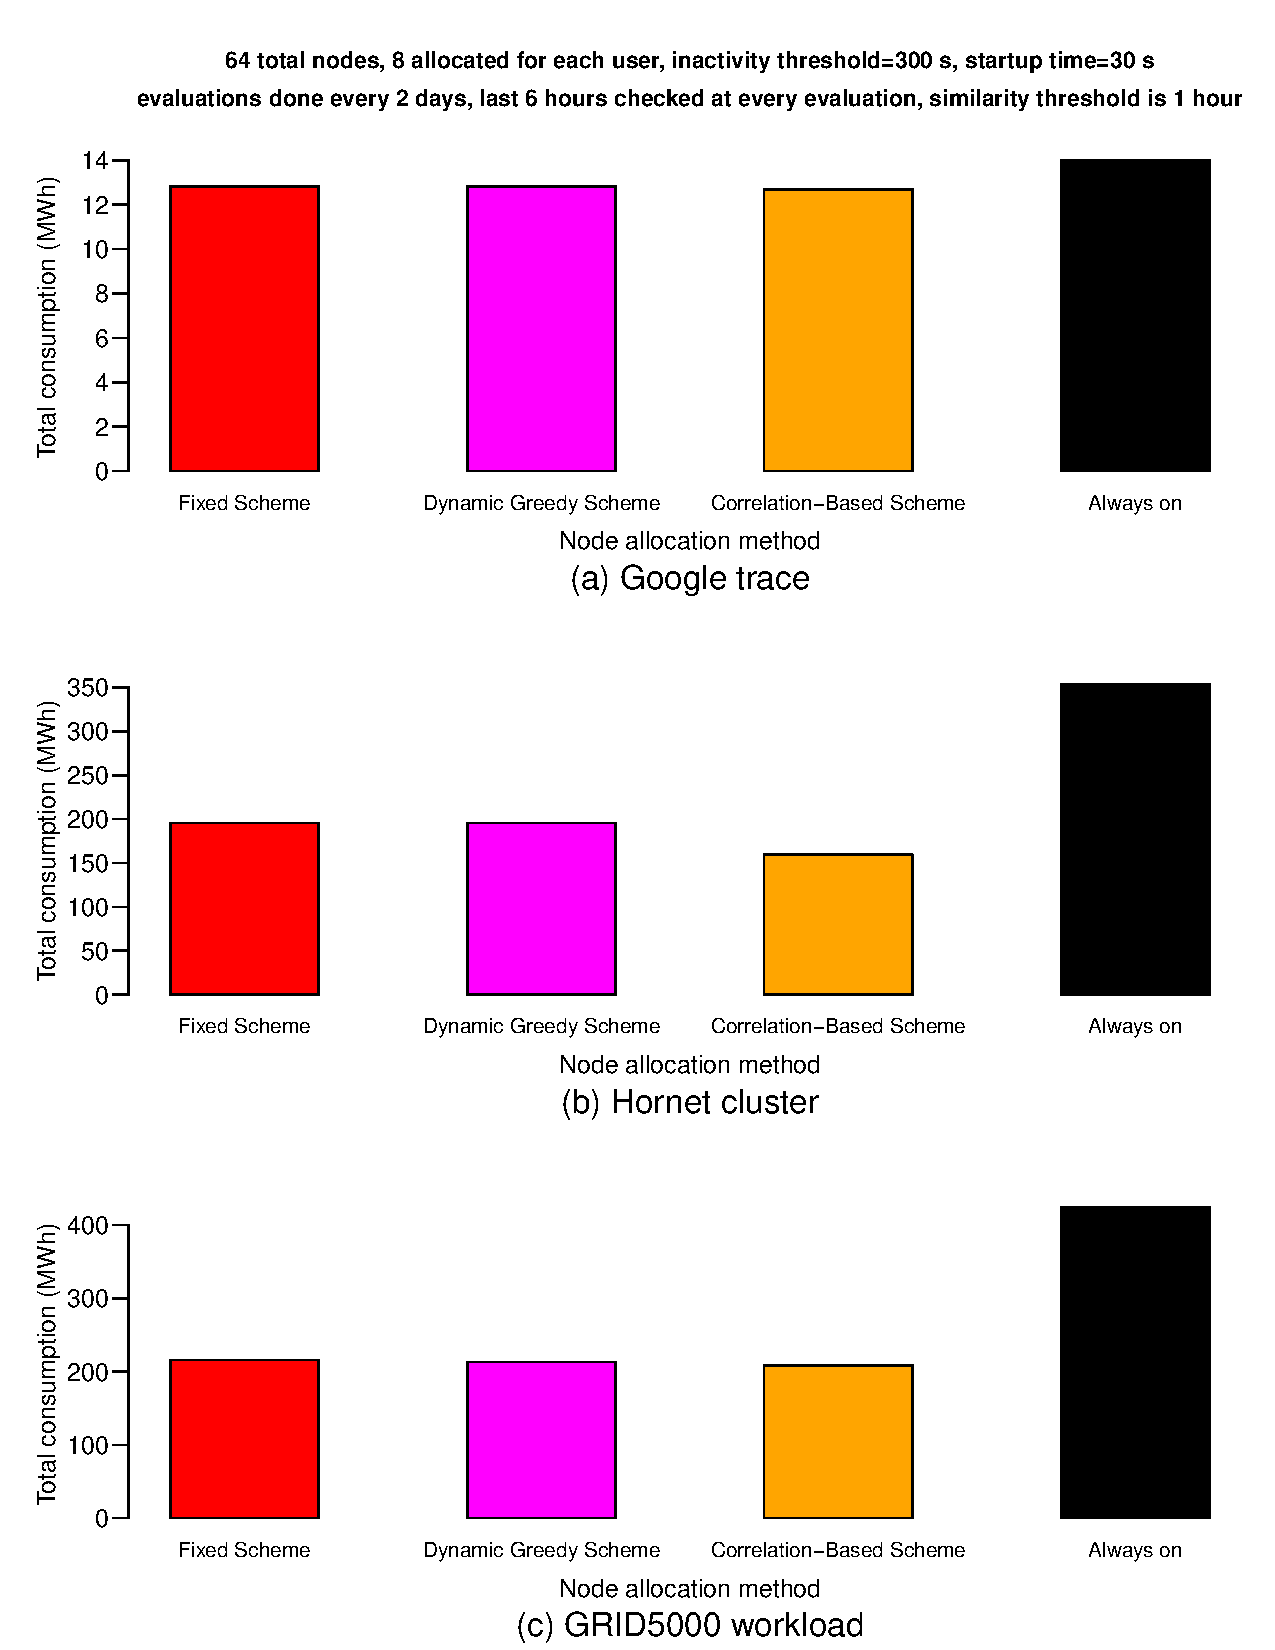
\includegraphics[width=\columnwidth,keepaspectratio]{FIG5.pdf}
\caption{Energy consumption comparison of methods}
\label{bigresult}
\end{figure}

Figure~\ref{bigresult} shows that, for the Google trace any of the methods would deliver the same amount
of energy savings and the percentage of energy savings is 8.4\% at its maximum. Google trace is a highly
I/O intensive workload and there are not many idle periods in the system. As a result, energy savings are
not significant. For Hornet cluster data and GRID5000 workload, we observe that all three workloads save
significant amount of energy. For both of these workloads, we see that Dynamic Greedy scheme does not
improve on energy consumption that much compared to the Fixed scheme. One of the main objectives of the
Dynamic Greedy scheme is to balance load across the storage system. As a result, balancing the load
across the system prevents further energy savings. Correlation-Based scheme provides slightly better energy
savings for GRID5000 workload and much better energy savings for Hornet cluster data. Hornet cluster is mostly
used by researchers working simultaneously on a project which potentially improves the correlation
between storage system users. For Hornet cluster data the energy savings are as high as 55\% and
for GRID5000 workload energy savings are as high as 50.9\%.

\subsection{Fixed Scheme}
We first evaluate the Fixed scheme, where one of the node allocation techniques (balancing, sequential,
random or groups) is chosen and kept active unless manually changed. We calculate the total
energy consumption, load balance and latency per access with 64 total nodes in the system,
where 8 nodes are allocated for each user. Figure~\ref{firstresult} shows how energy consumption, load balance
and latency per access change with each node allocation technique. \textit{Random} node allocation technique is
executed five times and the average result is reported, as it can yield to a different result
at each run. Due to space considerations, we show only the Google trace evaluations of the Fixed scheme,
as other workloads have similar results. 
 
\begin{figure}[!htbp]
\centering
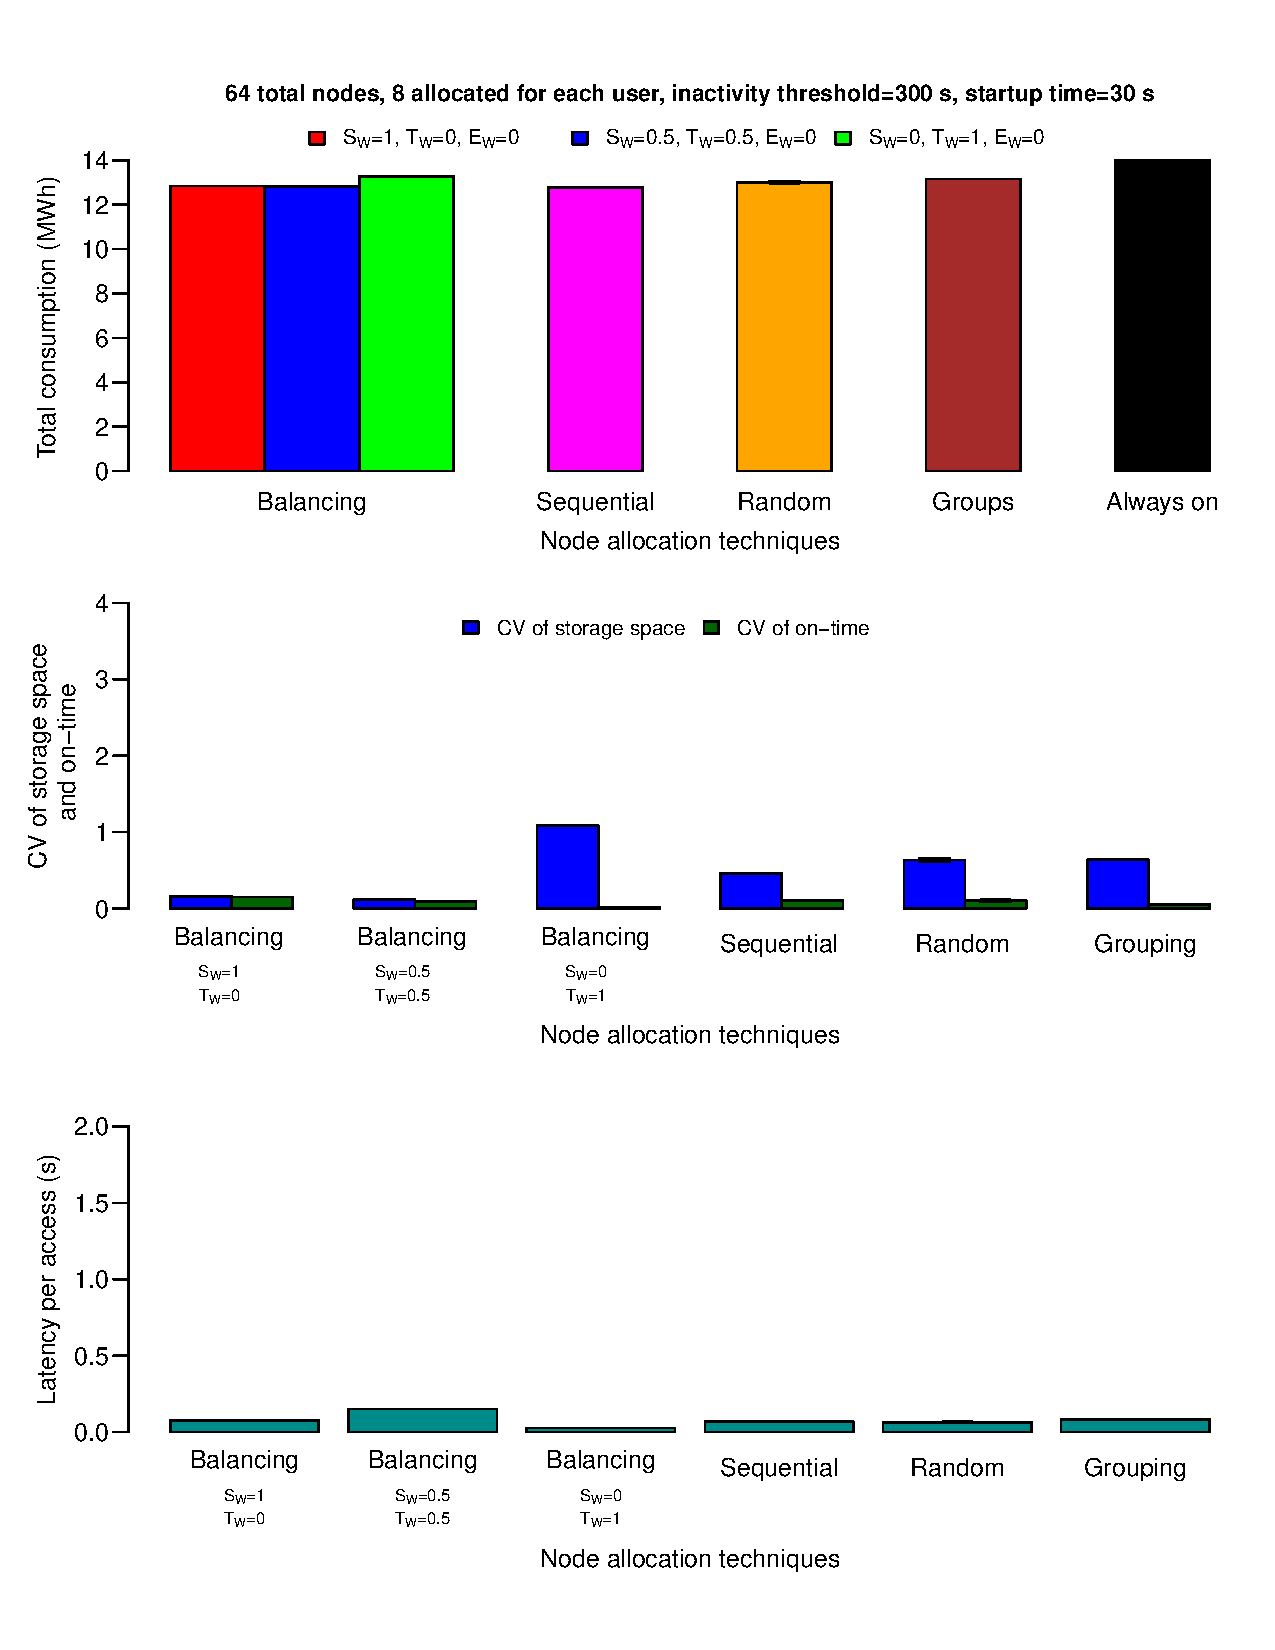
\includegraphics[width=\columnwidth,keepaspectratio]{FIG6.pdf}
\caption{Allocation technique vs energy consumption, load balance and latency per access (Fixed scheme - Google trace)}
\label{firstresult}
\end{figure}

As seen in Figure~\ref{firstresult}, each node allocation technique saves some amount of energy
compared to the stock case where there is no energy saving technique in place (system always on).
The percentage of savings is around 8.4\% for the Google trace. Google trace is highly intensive and as a
result, there are not that many idle periods in this workload. Therefore, energy savings are limited in
such a busy workload.
The amount of energy savings does not
vary much with different techniques. Balancing technique with on-time balancing weight ($T_W$) set to
one consumes slightly more energy compared to other techniques. The primary objective of balancing technique
with on-time balancing weight set to one is to balance the on-time of nodes across the storage system. We found
from the Google trace that majority of the storage system accesses are in the range of couple hundred seconds.
Google trace workload is already balanced initially in terms of node on-time; therefore, balancing technique
with on-time balancing weight set to one does not change the node allocations as much as other techniques do,
resulting in higher energy consumption.

However, the techniques do differ considerably in terms of balancing storage space and on-time. Second sub-plot in
Figure~\ref{firstresult} shows how the coefficient of variation (CV) of storage space and on-time across the storage nodes
vary with different node allocation techniques. As shown in the second sub-plot of Figure~\ref{firstresult}, the
balancing technique with non-zero storage space balancing weight ($S_W$) has smaller CV
of storage space across the storage nodes. Other techniques do not perform that well as their primary objective
is not to balance storage space across the storage nodes.

The balancing technique also performs well for balancing on-time of the storage nodes, as shown in the second sub-plot
of Figure~\ref{firstresult}. Balancing technique with time balancing weight ($T_W$) set to one has the smallest CV
of on-time across the storage nodes as expected.

The third sub-plot in Figure~\ref{firstresult} shows how the latency per access changes with each node allocation technique.
As we have mentioned previously, balancing technique with on-time balancing weight set to one does not change the node
allocations as much as other techniques do. As a result, that technique has the smallest latency per access. On the
other hand, balancing technique with both storage and on-time balancing weight set to 0.5 has the highest energy savings
compared to other techniques; increasing its latency per access. In general, we can see that all techniques have very
close latency per access values, usually around 0.1 seconds. 

\begin{figure}[!htbp]
\centering
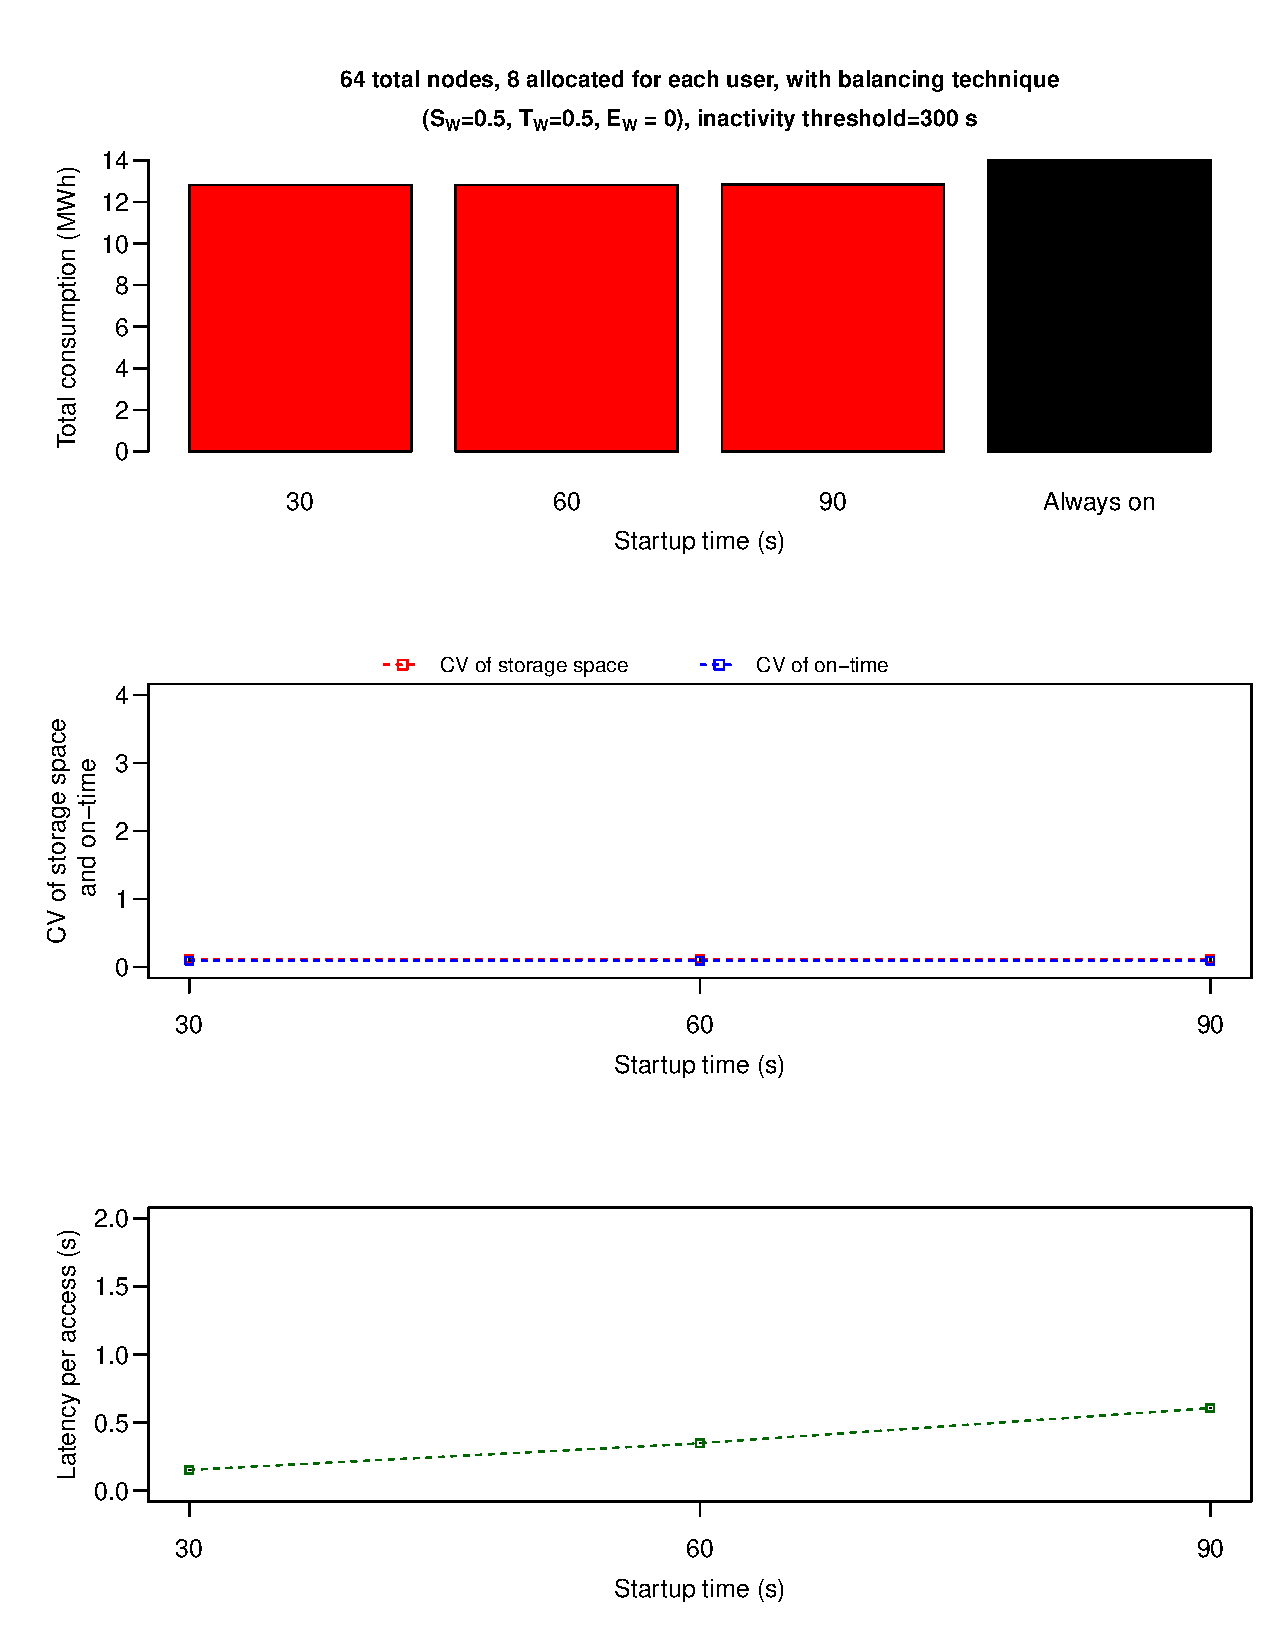
\includegraphics[width=\columnwidth,keepaspectratio]{FIG7.pdf}
\caption{The effect of varying the startup time (Fixed scheme - Google trace)}
\label{secondresult}
\end{figure}

\begin{figure}[!htbp]
\centering
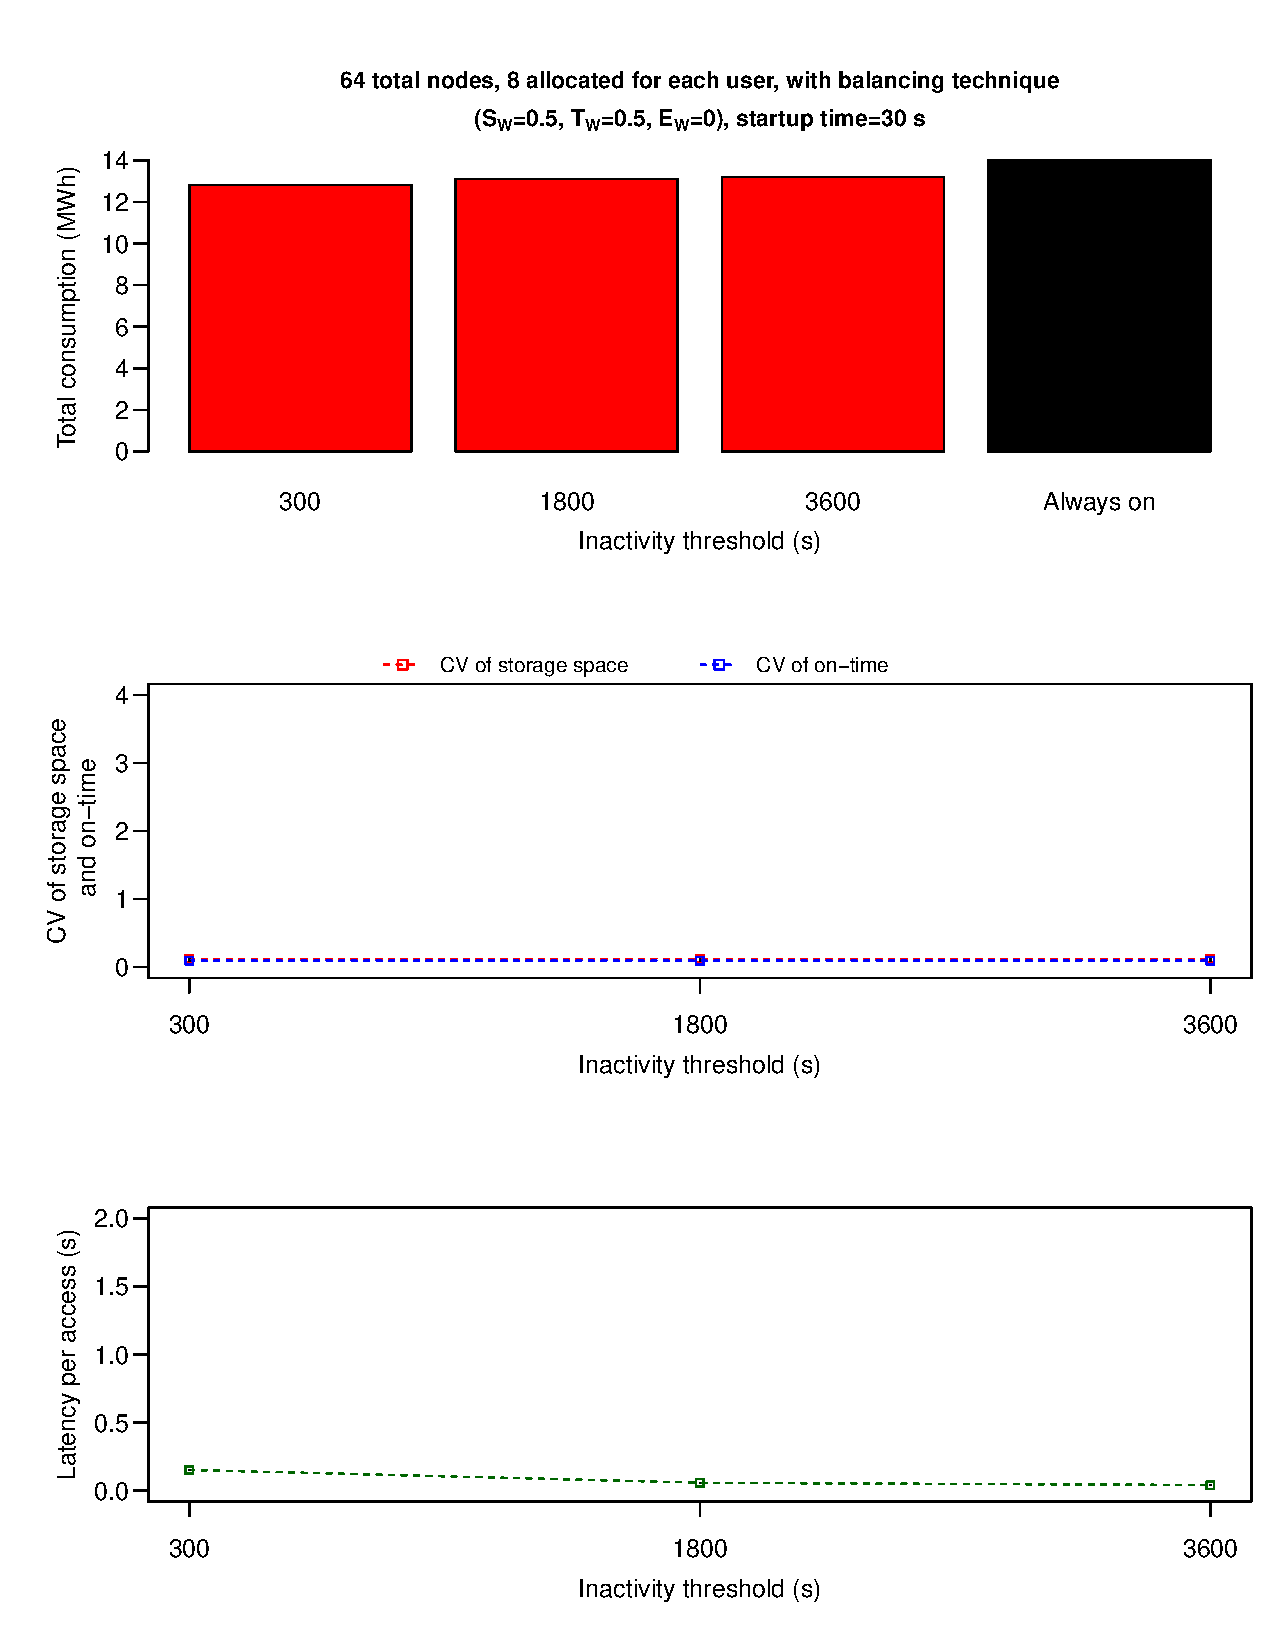
\includegraphics[width=\columnwidth,keepaspectratio]{FIG8.pdf}
\caption{The effect of varying the inactivity threshold (Fixed scheme - Google trace)}
\label{thirdresult}
\end{figure}

We also investigate how the total energy consumption, load balance and latency per access is affected by the changes in
the startup time and inactivity threshold. Figure~\ref{secondresult} shows the total energy consumption,
load balance and latency per access measurements while the startup time is varied between 30, 60 and 90 seconds. Similarly,
Figure~\ref{thirdresult} shows the total energy consumption, load balance and latency per access measurements while the
inactivity threshold is varied between 300, 1800 and 3600 seconds. As each technique is affected similarly by the changes
in the inactivity threshold and startup time, we only present results for the balancing technique with both storage space
and on-time balancing weights ($S_W$ and $T_W$) equal to 0.5 and energy consumption weight ($E_W$) equal to zero.

As we can see in both Figure~\ref{secondresult} and Figure~\ref{thirdresult}, changing the inactivity threshold or the
startup time has nearly no effect on the load balance. Changing the startup time does not affect the energy consumption
either. Figure~\ref{thirdresult} shows that increasing the inactivity threshold causes energy consumption to go up. When
the inactivity threshold is higher, it is less likely for a storage node to be turned-off for being idle longer
than this threshold. This causes the storage node to stay on for longer and consequently increases energy consumption.
Latency per access slightly increases as the startup time is increased. This is expected, since any access that is made
to a turned-off node will wait longer for that node to startup again. On the other hand, as the inactivity threshold is
increased, latency per access slightly decreases. In that case, the storage nodes are kept on for longer due to higher
inactivity threshold; which means that less storage system accesses will be made to a turned-off node.

\subsection{Dynamic Greedy Scheme}
In this section, we evaluate the Dynamic Greedy scheme and find out how effective it is in terms of energy consumption, 
load balance and latency per access. As discussed in Section~\ref{greedy}, \textit{evaluation points} and
\textit{control periods} are two important parameters of the Dynamic Greedy scheme. Dynamic Greedy scheme starts with
one of the four node allocation techniques we proposed (balancing, sequential, random or grouping) and changes between
these techniques at evaluation points, if necessary. We try to understand if the initial technique chosen has any effect
on the energy consumption, load balance or latency. We also analyze the effect of varying evaluation points and
control periods on the energy consumption, load balance and latency per access.

To start with, we test the Dynamic Greedy scheme with varying storage-space, on-time and energy consumption weights
($S_W$, $T_W$ and $E_W$) where the total number of storage nodes in the system is 64 and the number of nodes allocated
for each user is 8, as shown in Figure~\ref{fourthresult}. The evaluations are done every 2 days and the storage
accesses in the last 6 hours are checked. Each measurement is the average of five runs. Due to space considerations, we
show only the Hornet cluster evaluations of the Dynamic Greedy scheme, as other workloads have similar results.

\begin{figure}[!htbp]
\centering
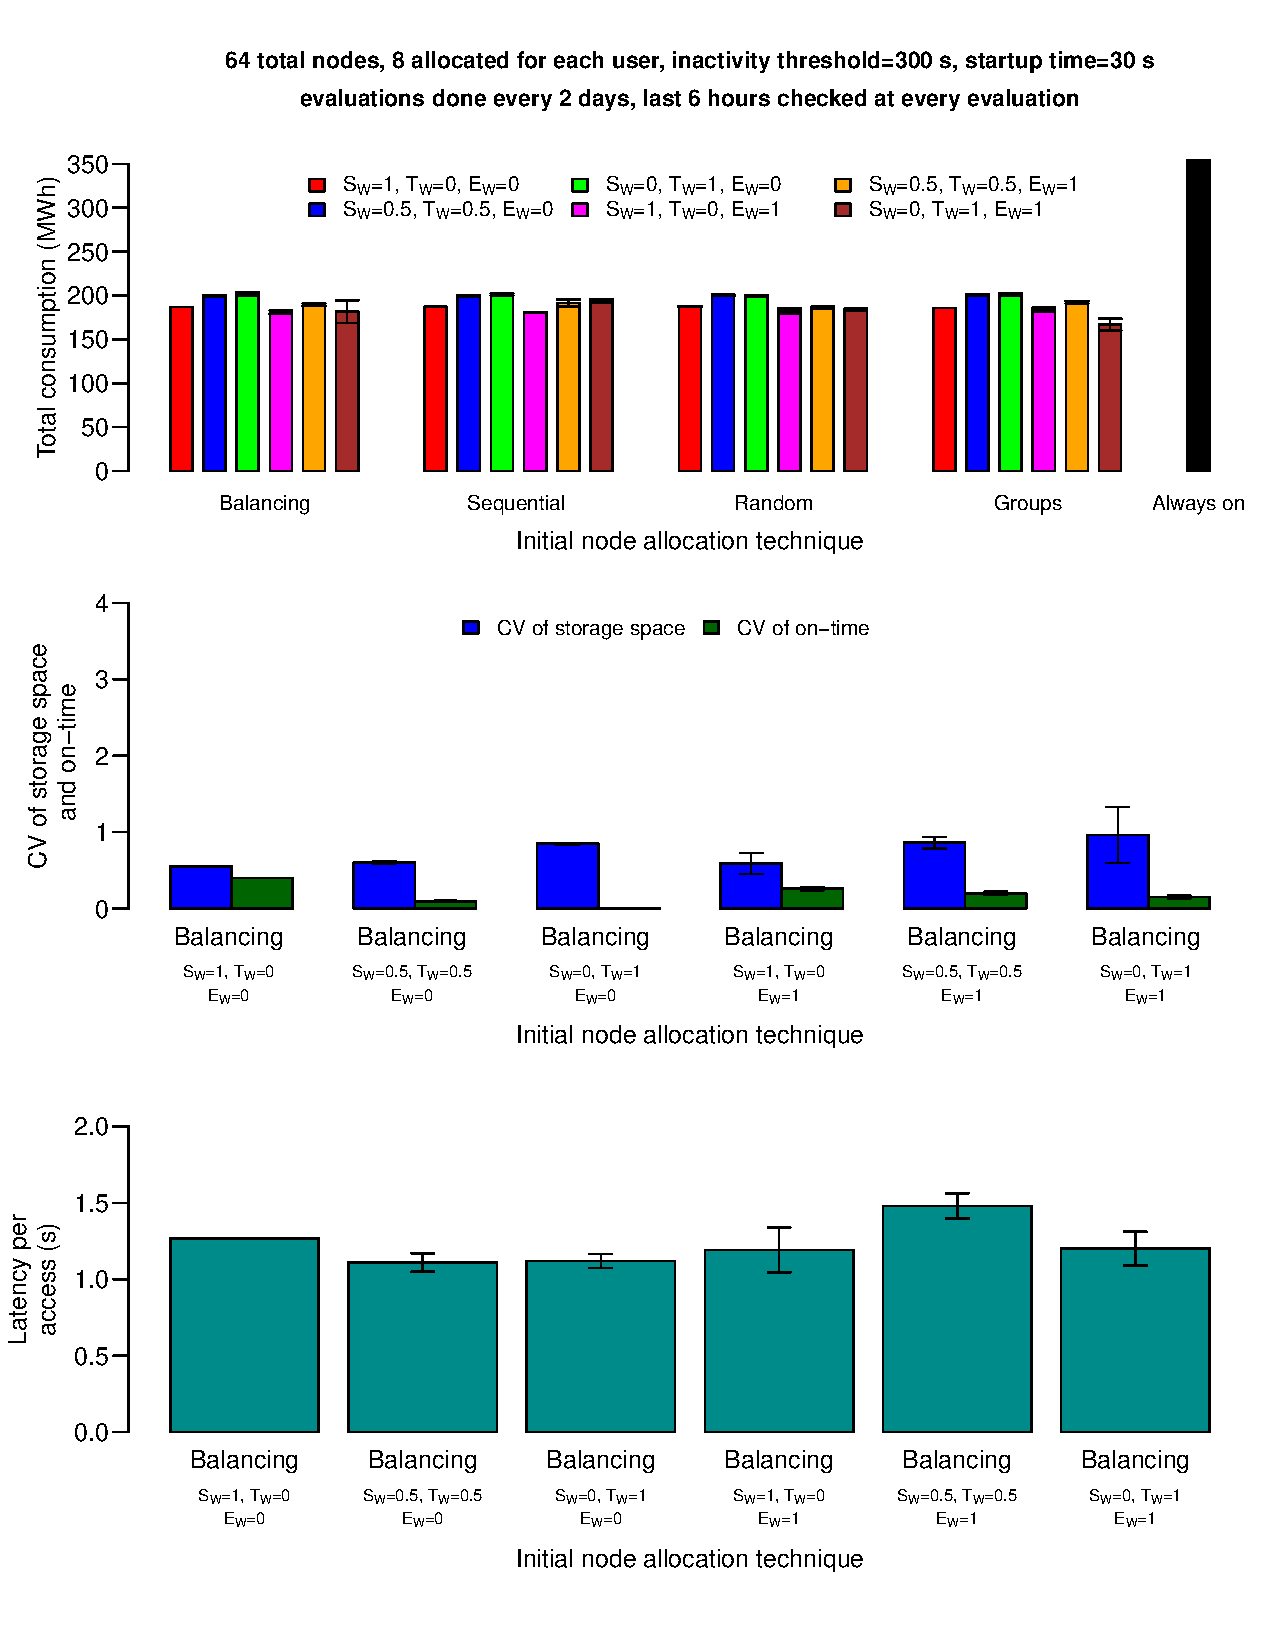
\includegraphics[width=\columnwidth,keepaspectratio]{FIG9.pdf}
\caption{Initial technique vs energy consumption, load balance and latency per access (Dynamic Greedy scheme - Hornet cluster)}
\label{fourthresult}
\end{figure}

Figure~\ref{fourthresult} shows that the Dynamic Greedy scheme saves a considerable amount of energy regardless of
which node allocation technique is chosen initially. The percentage of energy savings are between 43.4\% and 52\%
for varying storage space, on-time and energy weights. Regardless of which technique is initially chosen, we can
see that cases where the energy consumption weight ($E_W$) is set to one consume less energy compared to the cases
where the energy consumption weight is set to zero. Another observation we can make is that the cases where the
on-time balancing weight ($T_W$) is non-zero and energy consumption weight ($E_W$) is set to zero consume more
energy. In the Hornet cluster workload, storage system access lengths vary significantly. As a result,
while trying to balance the on-time across the storage nodes, it is more likely to transfer users from one node
to another. Storage space usage among the users vary as well, though not as much as the access lengths.

In the second sub-plot of Figure~\ref{fourthresult}, we can see how the CVs of storage space and
on-time change when the storage space, on-time and energy consumption weights are varied. Regardless of
which allocation technique is chosen initially (balancing, sequential, random or grouping) the CVs of the
storage space and on-time are similar. Therefore, we only show the results for cases where balancing technique
is the initially chosen technique. We can see that the CV of the storage space is the smallest when the storage space
balancing weight ($S_W$) is set to one, regardless of the energy consumption weight ($E_W$). As the on-time
balancing weight ($T_W$) is increased, the CV of the storage space increases as well. The same holds true
for the CV of the on-time. When the on-time balancing weight ($T_W$) is set to one, the CV of the on-time
is the smallest regardless of the energy consumption weight ($E_W$). As the storage space balancing
weight ($S_W$) is increased, the CV of the on-time increases as well.

We can see how latency per storage access changes with varying storage space, on-time and energy consumption
weights in the third sub-plot of Figure~\ref{fourthresult}. Again, as it does not matter which allocation technique
is initially chosen, we only show the results for cases where the balancing technique is the initially chosen
technique. The latency
measurements are almost the inverse of the energy consumption measurements in the first sub-plot of
Figure~\ref{fourthresult}. In the first sub-plot of Figure~\ref{fourthresult}, we have seen that when the energy
consumption weight ($E_W$) is set to one, the energy consumption goes down. This means that a storage access
will most likely be made on a turned-off node, increasing latency per access. We have also seen in the
first sub-plot of Figure~\ref{fourthresult} that when on-time balancing weight is non-zero and the energy
consumption weight ($E_W$) is set to zero, the energy savings are less. This will in turn
decrease the chance of an access to be made to a turned-off node, decreasing latency per access.

\begin{figure}[!htbp]
\centering
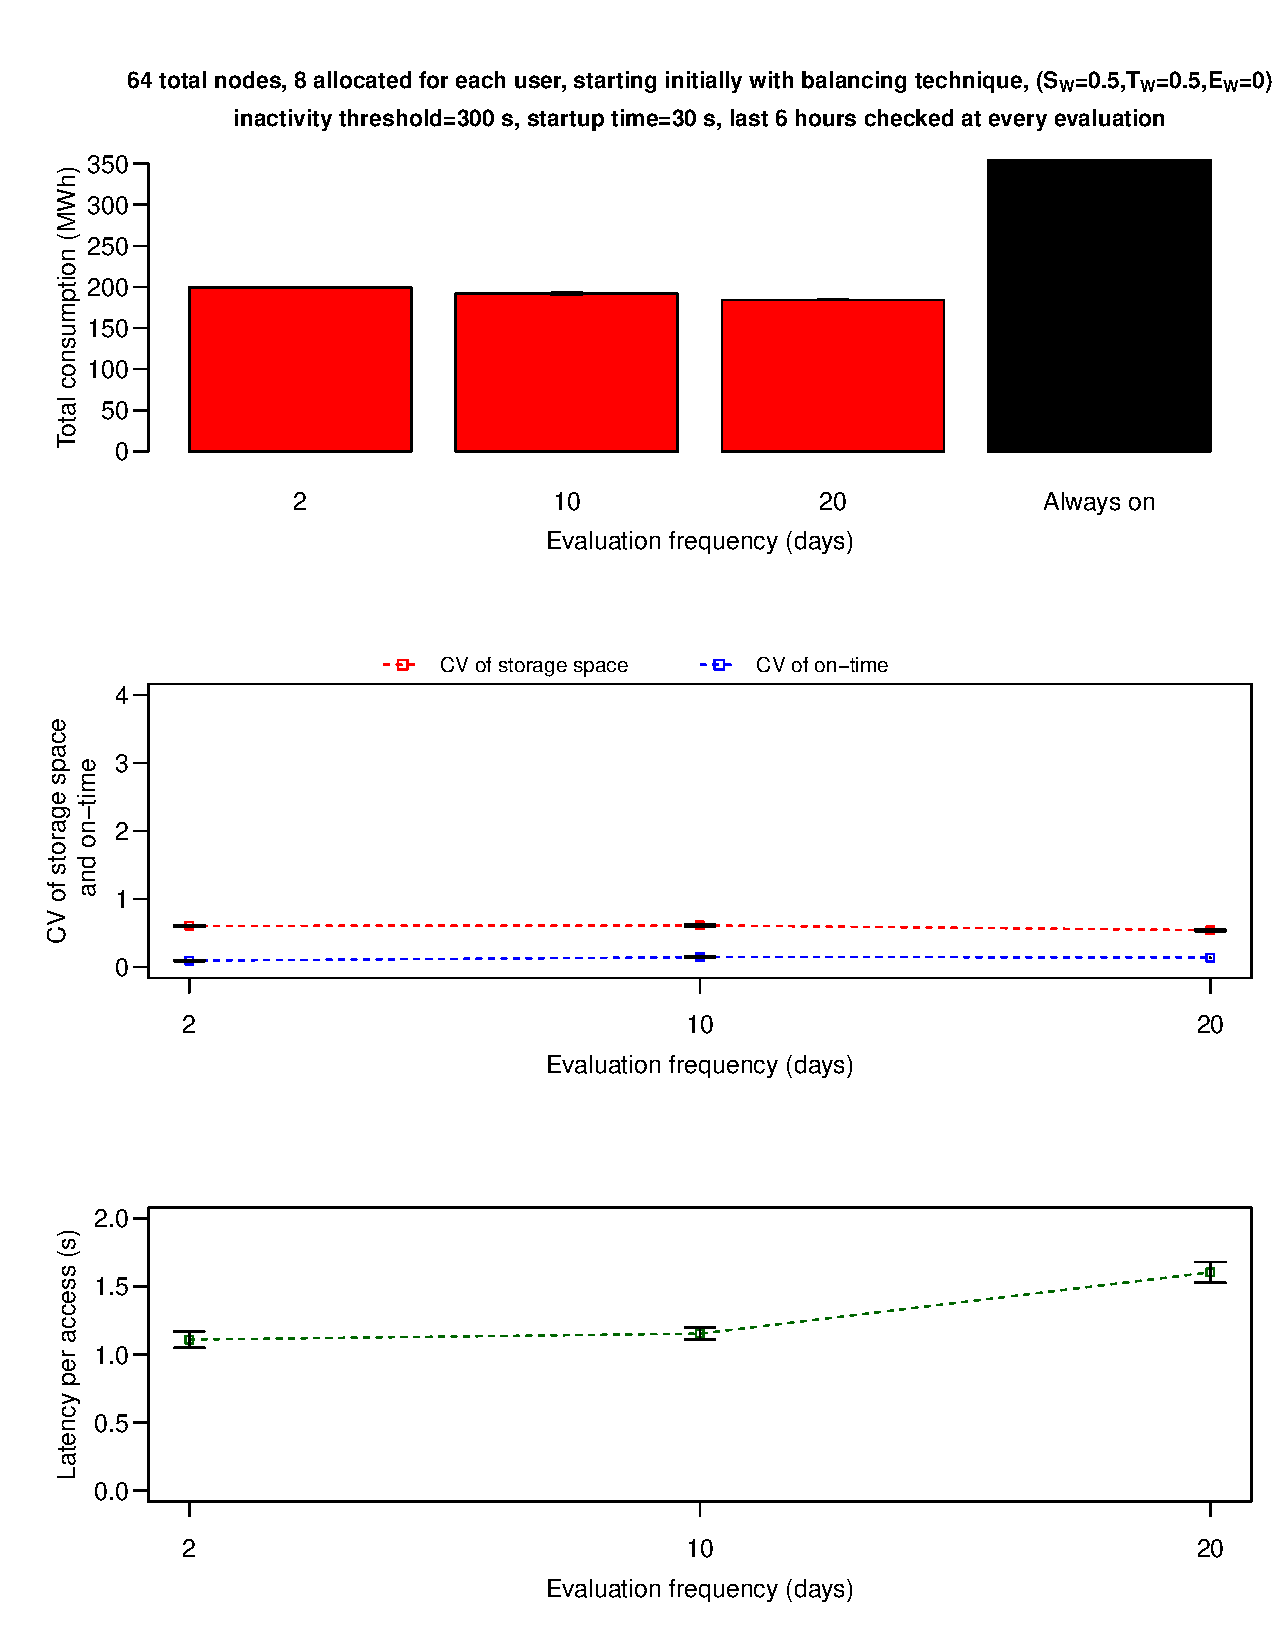
\includegraphics[width=\columnwidth,keepaspectratio]{FIG10.pdf}
\caption{The effect of varying the evaluation frequency (Dynamic Greedy scheme - Hornet cluster)}
\label{fifthresult}
\end{figure}

We now look at the effect of varying the evaluation frequency on the total energy consumption,
load balance and latency per access. The evaluation frequency is varied between 2, 10 and 20 days
and the control period is fixed at 6 hours. Since the initial allocation technique does not change
the results, we initially start with the balancing technique with both storage space and on-time
balancing weights ($S_W$ and $T_W$) set to 0.5 and energy consumption weight ($E_W$) set to zero.
As shown in Figure~\ref{fifthresult}, total energy consumption goes down as the evaluation frequency
becomes longer. When the evaluation frequency is longer, our algorithms have more knowledge about
the state of the storage system. Therefore, more intelligent decisions are made for reducing energy
consumption. We also see that the CVs of the storage space and on-time is almost not affected by
the evaluation frequency. In the third sub-plot of Figure~\ref{fifthresult}, we observe that latency
per access increases as the evaluation frequency becomes longer. This is expected, as longer evaluation
frequency reduces energy consumption by turning off storage nodes more often. 

\begin{figure}[!htbp]
\centering
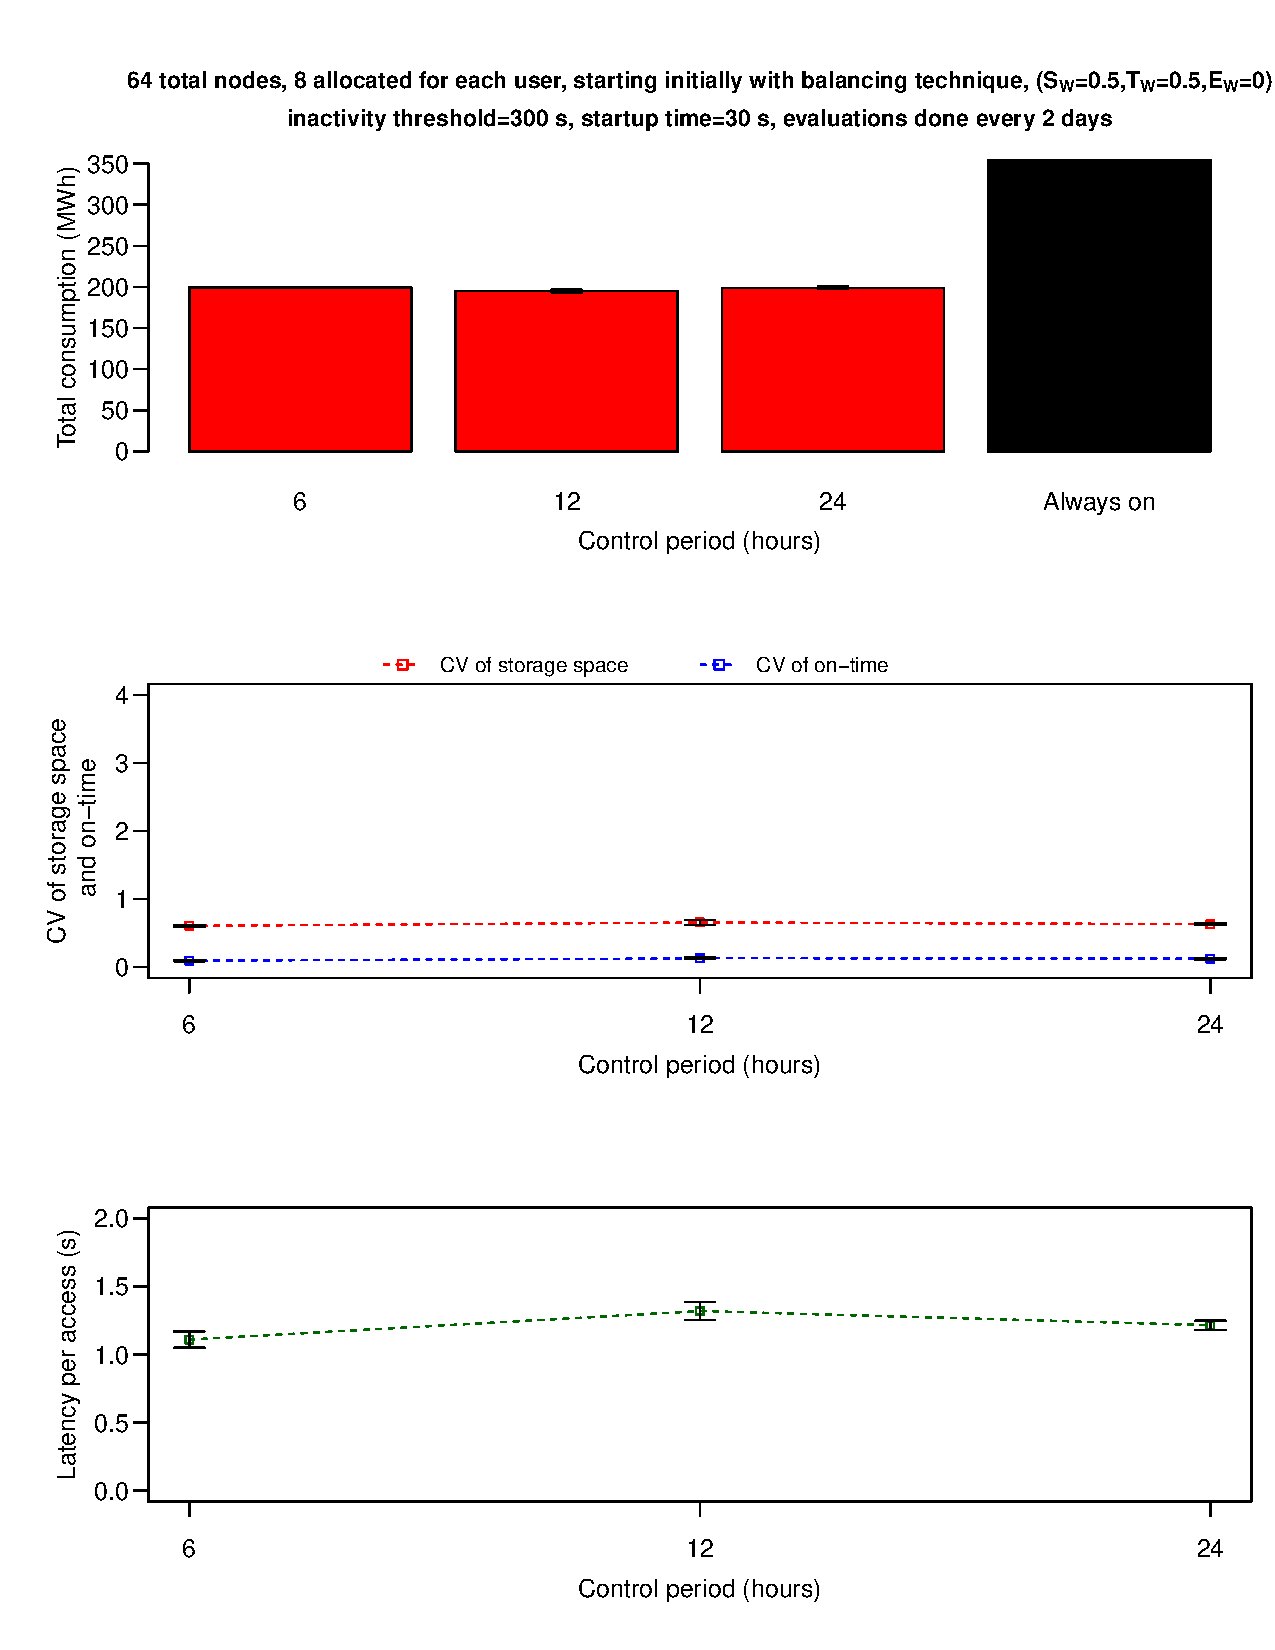
\includegraphics[width=\columnwidth,keepaspectratio]{FIG11.pdf}
\caption{The effect of varying the control period (Dynamic Greedy scheme - Hornet cluster)}
\label{sixthresult}
\end{figure}

Figure~\ref{sixthresult} shows the effect of varying the control period (between 6, 12 and 24 hours)
on the total energy consumption, load balance and latency per access. In this test case the evaluation
frequency is fixed at 2 days. The results in Figure~\ref{sixthresult} indicate that varying the control
period does not affect the total energy consumption, load balance or latency per access.

\subsection{Correlation-Based Scheme}
In this section, we evaluate the Correlation-Based scheme and find out how effective it is in terms of energy consumption,
load balance and latency per access. Correlation-Based scheme starts with one of the four node allocation
techniques (balancing, sequential, random or grouping) similar to the Dynamic Greedy scheme. Unlike the Dynamic
Greedy scheme, it checks the correlations between users at evaluation points and allocates the same storage
nodes for correlated users instead of changing the initial node allocation technique. As a matter of fact,
initial node allocation technique is used if only a user accesses the storage system for the first time.
During the following tests, we also try to understand if the initial technique chosen has any effect on the
energy consumption, load balance or latency per access.

Correlation-Based scheme also has \textit{evaluation point} and \textit{control period} parameters. We have
already shown the effect of varying these two parameters for the Dynamic Greedy scheme; therefore, we are not
repeating the same tests for Correlation-Based scheme. \textit{Similarity threshold} is a parameter that
is unique to the Correlation-Based scheme. We look at the effect of this parameter on the energy consumption,
load balance and latency per access as well.

To start with, we test the Correlation-Based scheme with different initial techniques, where the total number of
storage nodes in the system is 64 and the number of nodes allocated for each user is 8, as shown in 
Figure~\ref{seventhresult}. The evaluations are done every 2 days and the storage accesses in the last 6 hours
are checked. Each measurement is the average of five runs. Since energy consumption weight is not important
in Correlation-Based scheme, it is fixed at zero in this test case. Due to space considerations, we
show only the GRID5000 workload evaluations of the Correlation-Based scheme, as other workloads have similar
results.

\begin{figure}[!htbp]
\centering
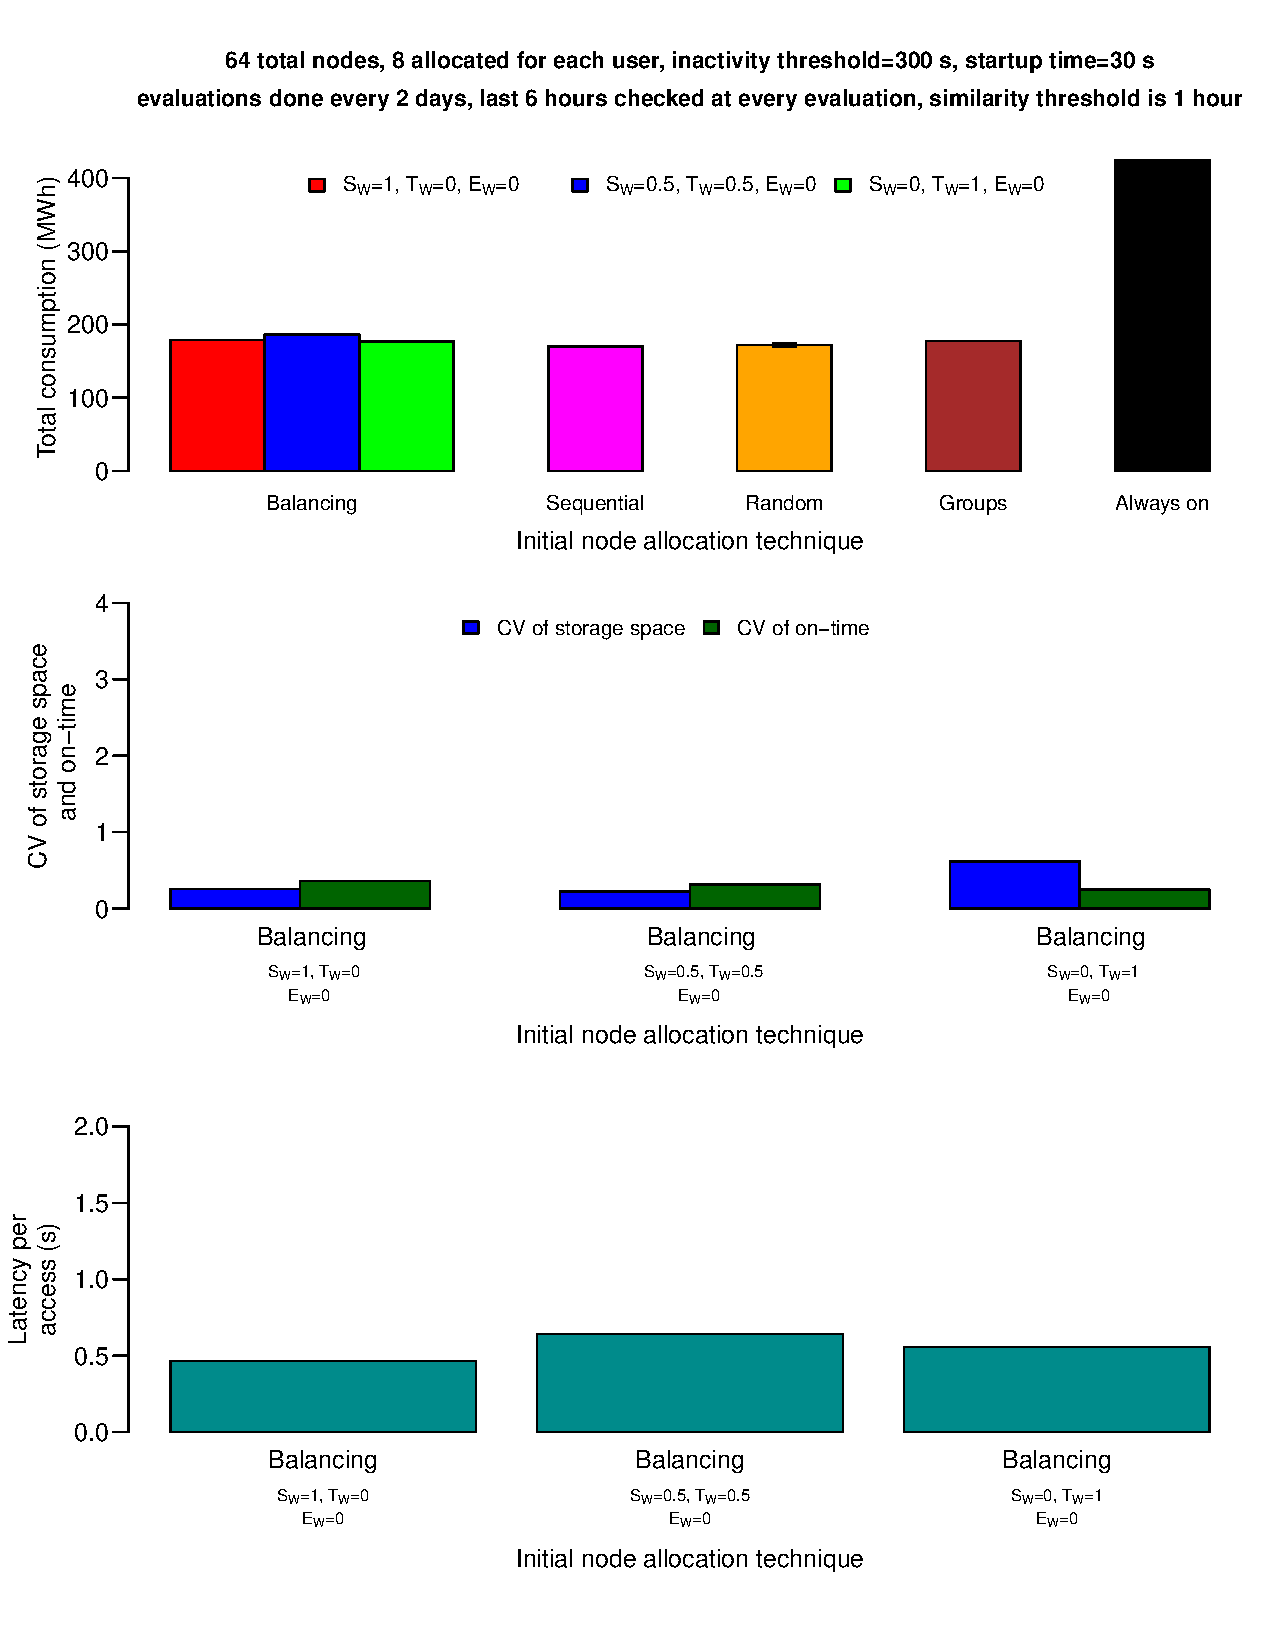
\includegraphics[width=\columnwidth,keepaspectratio]{FIG12.pdf}
\caption{Initial technique vs energy consumption, load balance and latency (Correlation-Based scheme -
 GRID5000 workload)}
\label{seventhresult}
\end{figure}

Figure~\ref{seventhresult} shows that Correlation-Based Scheme saves more than half of the energy consumed
in the stock case regardless of the initial node allocation technique. The percentage of energy savings
are as high as 60\%. We observe that the initial technique chosen does not have a significant effect on
the energy consumption.

The CVs of the storage space and on-time are shown in the second sub-plot of Figure~\ref{seventhresult}.
As the initial technique chosen for the Correlation-Based scheme does not really matter, we show
results for the balancing technique with varying storage-space and on-time balancing weights. As the
storage space balancing weight ($S_W$) is increased, the CV of the storage space
decreases. The same is true for on-time.

The third sub-plot in Figure~\ref{seventhresult} shows how latency per access is affected when the initial
technique is balancing with varying storage-space and on-time balancing weights. In GRID5000 workload, the
storage space usage of users are close to each other. Therefore balancing technique with storage-space
balancing weight set to one will not effect the node allocations as much as other techniques do. We observed
that GRID5000 workload havs accesses of varying lengths, particularly
until the first evaluation point. As a result, if both the storage space balancing and on-time weight are set
to 0.5, then the algorithm will not try to break already balanced storage-space distribution, while at the
same time trying to balance on-time. This will in turn result in more transfers and consequently more latency.
This feature of the GRID5000 workload is similar to that of Google trace in Figure~\ref{firstresult}, except
that Google trace had varying storage space usage among the users where access lenghts did not vary that much.

\begin{figure}[!htbp]
\centering
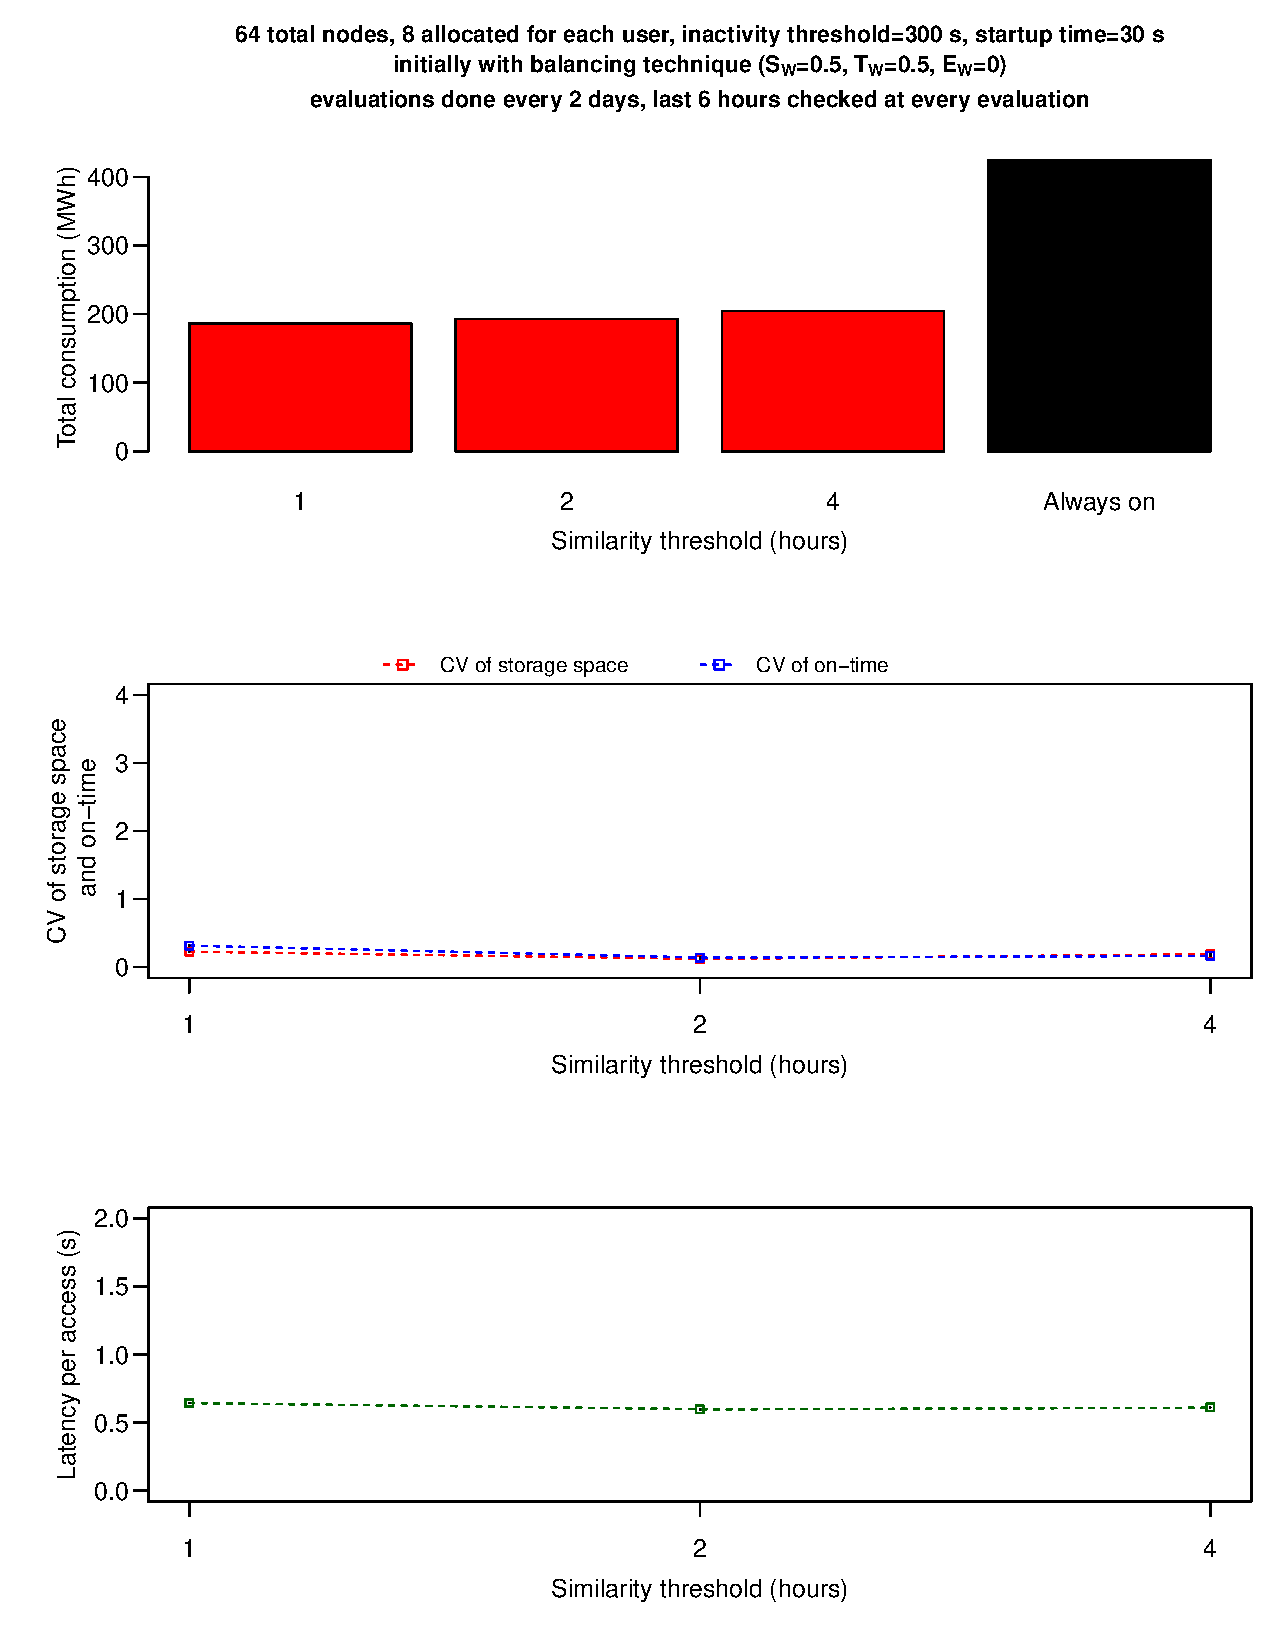
\includegraphics[width=\columnwidth,keepaspectratio]{FIG13.pdf}
\caption{The effect of varying the similarity threshold (Correlation-Based scheme - GRID5000 workload)}
\label{eightthresult}
\end{figure} 

Figure~\ref{eightthresult} shows the effect of varying the similarity threshold on the total energy
consumption, load balancing and latency per access. Evaluations are done every 2 days and the last 6 hours
are checked at every evaluation. Balancing technique with both storage space and on-time balancing
weights set to 0.5 is used initially. Similar to the inactivity threshold, varying the
similarity threshold has almost no effect on the standard devations of the storage space and on-time
or latency per access. When the similarity threshold is increased, total energy consumption
increases slightly. The higher the similarity threshold is, the less likely it is to find correlated
users. As a result, energy consumption goes up with higher similarity threshold.

\subsection{Validating Mathematical Model}
\label{validate_model}
We have validated the mathematical model presented in Section~\ref{model} against the
experimental results of our approach using data from Hornet HPC system. We can estimate the energy
consumption, load balancing and latency per access values for each workload
by using the mathematical model presented in Section~\ref{model}. We validate
the mathematical model using the subset of test parameters as shown in
Table~\ref{tbl:validate_params}.
For brevity, we show only the Hornet data, though the other workloads show similar results.
For the Hornet data that we show here for this validation, we have primarily used a Generalized
Extreme Value interjob arrival model - i.e.
$F(t) = e^{-g(t)},\ \ where\ \ g(t)\ \ =\ \ [{1 + (\frac{t - \mu}{\sigma}) * \xi}]^{\frac{-1}{\xi}}$
and $\xi,\ \ \mu$ and $\sigma$ are distribution parameters.

\begin{table}[!htbp]
 \begin{center}
  \begin{tabular}{|l|l|} \hline
Test Parameter & Values \\ \hline
Total number of nodes          & 64 \\ \hline
Number of nodes allocated        & 8 \\
for each user              & \\ \hline
Allocation methods           & Fixed, Dynamic Greedy, Correlation-Based \\ \hline
Low-energy mode             & Turn Off \\ \hline
Inactivity threshold          & 300 s \\ \hline
Startup time              & 30 s \\ \hline
Similarity threshold          & 3600 s \\ \hline
Storage space and on-time        & 0.5, 0.5, 0 \\
balancing weights            & \\ \hline
Power consumption per node       & 300 W \\ \hline
Workloads                        & Hornet \\ \hline
  \end{tabular}
 \end{center}
 \caption{Mathematical Model Validation Parameters}
 \label{tbl:validate_params}
\end{table}

Tables~\ref{tbl:validate_results_fixed},~\ref{tbl:validate_results_dynamic} and ~\ref{tbl:validate_results_corr} show
that the mathematical model we presented is able to estimate the test result parameters (CV of storage space, CV of on-time
, energy cost and latency per access) accurately in most
cases. The storage space usage of a user per storage node does not change over time; therefore, the chance of
estimating it accurately is high. Our model estimates on-time value and energy consumption of each storage node accurately
as well, as estimating them involves all of the parameters captured by our model except storage space usage.
Latency per access is highly dependent on the arrival rate of \textit{interarrivals} and our model does the best attempt to
capture these interarrivals in order to estimate the latency per access.

\begin{table}[!htbp]
 \begin{center}
 \resizebox{\textwidth}{!}{%
  \begin{tabular}{lcccccccc} \hline
\multicolumn{1}{|c}{} & \multicolumn{4}{c|}{Balancing} & \multicolumn{4}{c|}{Sequential}\\ \hline
\multicolumn{1}{|c}{} & \multicolumn{1}{|c}{Storage} & \multicolumn{1}{c}{On-time} & \multicolumn{1}{c}{Energy} & \multicolumn{1}{c|}{Latency per} & \multicolumn{1}{c}{Storage} & \multicolumn{1}{c}{On-time} & \multicolumn{1}{c}{Energy} & \multicolumn{1}{c|}{Latency per} \\
\multicolumn{1}{|c}{} & \multicolumn{1}{|c}{CV} & \multicolumn{1}{c}{CV} & \multicolumn{1}{c}{cost (MWh)} & \multicolumn{1}{c|}{access (s)} & \multicolumn{1}{c}{CV} & \multicolumn{1}{c}{CV} & \multicolumn{1}{c}{cost (MWh)} & \multicolumn{1}{c|}{access (s)} \\ \hline
\multicolumn{1}{|l|}{Simulation} & 0.539 & 0.312 & 195.65 & \multicolumn{1}{c|}{1.0348} & 0.757 & 0.382 & 181.01 & \multicolumn{1}{c|}{1.1833} \\ 
\multicolumn{1}{|l|}{Model} & 0.543 & 0.3145 & 195.62 & \multicolumn{1}{c|}{1.1657} & 0.7628 & 0.3849 & 180.93 & \multicolumn{1}{c|}{1.1669} \\
\multicolumn{1}{|l|}{Error} & 0.74\% & 0.80\% & 0.02\% & \multicolumn{1}{c|}{12.65\%} & 0.77\% & 0.76\% & 0.04\% & \multicolumn{1}{c|}{1.39\%} \\ \hline
& & & & & & & & \\ \hline
\multicolumn{1}{|c}{} & \multicolumn{4}{c|}{Random} & \multicolumn{4}{c|}{Groups}\\ \hline
\multicolumn{1}{|c}{} & \multicolumn{1}{|c}{Storage} & \multicolumn{1}{c}{On-time} & \multicolumn{1}{c}{Energy} & \multicolumn{1}{c|}{Latency per} & \multicolumn{1}{c}{Storage} & \multicolumn{1}{c}{On-time} & \multicolumn{1}{c}{Energy} & \multicolumn{1}{c|}{Latency per} \\
\multicolumn{1}{|c}{} & \multicolumn{1}{|c}{CV} & \multicolumn{1}{c}{CV} & \multicolumn{1}{c}{cost (MWh)} & \multicolumn{1}{c|}{access (s)} & \multicolumn{1}{c}{CV} & \multicolumn{1}{c}{CV} & \multicolumn{1}{c}{cost (MWh)} & \multicolumn{1}{c|}{access (s)} \\ \hline
\multicolumn{1}{|l|}{Simulation} & 0.9 & 0.394 & 179.81 & \multicolumn{1}{c|}{1.5673} & 1.129 & 0.351 & 183.78 & \multicolumn{1}{c|}{1.0367} \\ 
\multicolumn{1}{|l|}{Model} & 0.9069 & 0.3973 & 179.753 & \multicolumn{1}{c|}{1.2496} & 1.1381 & 0.3539 & 183.711 & \multicolumn{1}{c|}{1.0539} \\
\multicolumn{1}{|l|}{Error} & 0.77\% & 0.84\% & 0.03\% & \multicolumn{1}{c|}{20.27\%} & 0.81\% & 0.83\% & 0.04\% & \multicolumn{1}{c|}{1.66\%} \\ \hline
  \end{tabular}}
 \end{center}
 \caption{Mathematical Model Validation Results for Fixed Scheme}
 \label{tbl:validate_results_fixed}
\end{table}

\begin{table}[!htbp]
 \begin{center}
 \resizebox{\textwidth}{!}{%
  \begin{tabular}{lcccccccc} \hline
\multicolumn{1}{|c}{} & \multicolumn{4}{c|}{Starts with Balancing} & \multicolumn{4}{c|}{Starts with Sequential}\\ \hline
\multicolumn{1}{|c}{} & \multicolumn{1}{|c}{Storage} & \multicolumn{1}{c}{On-time} & \multicolumn{1}{c}{Energy} & \multicolumn{1}{c|}{Latency per} & \multicolumn{1}{c}{Storage} & \multicolumn{1}{c}{On-time} & \multicolumn{1}{c}{Energy} & \multicolumn{1}{c|}{Latency per} \\
\multicolumn{1}{|c}{} & \multicolumn{1}{|c}{CV} & \multicolumn{1}{c}{CV} & \multicolumn{1}{c}{cost (MWh)} & \multicolumn{1}{c|}{access (s)} & \multicolumn{1}{c}{CV} & \multicolumn{1}{c}{CV} & \multicolumn{1}{c}{cost (MWh)} & \multicolumn{1}{c|}{access (s)} \\ \hline
\multicolumn{1}{|l|}{Simulation} & 0.605 & 0.0932 & 199.36 & \multicolumn{1}{c|}{1.11008} & 0.6186 & 0.0956 & 199.273 & \multicolumn{1}{c|}{1.12687} \\
\multicolumn{1}{|l|}{Model} & 0.6031 & 0.1006 & 199.913 & \multicolumn{1}{c|}{1.0424} & 0.6142 & 0.1 & 200.254 & \multicolumn{1}{c|}{0.9944} \\
\multicolumn{1}{|l|}{Error} & 0.31\% & 7.94\% & 0.28\% & \multicolumn{1}{c|}{6.1\%} & 0.71\% & 4.6\% & 0.49\% & \multicolumn{1}{c|}{11.76\%} \\ \hline
& & & & & & & & \\ \hline
\multicolumn{1}{|c}{} & \multicolumn{4}{c|}{Starts with Random} & \multicolumn{4}{c|}{Starts with Groups}\\ \hline
\multicolumn{1}{|c}{} & \multicolumn{1}{|c}{Storage} & \multicolumn{1}{c}{On-time} & \multicolumn{1}{c}{Energy} & \multicolumn{1}{c|}{Latency per} & \multicolumn{1}{c}{Storage} & \multicolumn{1}{c}{On-time} & \multicolumn{1}{c}{Energy} & \multicolumn{1}{c|}{Latency per} \\
\multicolumn{1}{|c}{} & \multicolumn{1}{|c}{CV} & \multicolumn{1}{c}{CV} & \multicolumn{1}{c}{cost (MWh)} & \multicolumn{1}{c|}{access (s)} & \multicolumn{1}{c}{CV} & \multicolumn{1}{c}{CV} & \multicolumn{1}{c}{cost (MWh)} & \multicolumn{1}{c|}{access (s)} \\ \hline
\multicolumn{1}{|l|}{Simulation} & 0.614 & 0.0926 & 200.199 & \multicolumn{1}{c|}{1.14529} & 0.63 & 0.086 & 200.558 & \multicolumn{1}{c|}{1.09082} \\
\multicolumn{1}{|l|}{Model} & 0.6092 & 0.0923 & 199.577 & \multicolumn{1}{c|}{1.022} & 0.6382 & 0.08 & 201.176 & \multicolumn{1}{c|}{1.0311} \\
\multicolumn{1}{|l|}{Error} & 0.78\% & 0.32\% & 0.31\% & \multicolumn{1}{c|}{10.76\%} & 1.3\% & 6.98\% & 0.31\% & \multicolumn{1}{c|}{5.47\%} \\ \hline
  \end{tabular}}
 \end{center}
 \caption{Mathematical Model Validation Results for Dynamic Greedy Scheme}
 \label{tbl:validate_results_dynamic}
\end{table}

\begin{table}[!htbp]
 \begin{center}
 \resizebox{\textwidth}{!}{%
  \begin{tabular}{lcccccccc} \hline
\multicolumn{1}{|c}{} & \multicolumn{4}{c|}{Starts with Balancing} & \multicolumn{4}{c|}{Starts with Sequential}\\ \hline
\multicolumn{1}{|c}{} & \multicolumn{1}{|c}{Storage} & \multicolumn{1}{c}{On-time} & \multicolumn{1}{c}{Energy} & \multicolumn{1}{c|}{Latency per} & \multicolumn{1}{c}{Storage} & \multicolumn{1}{c}{On-time} & \multicolumn{1}{c}{Energy} & \multicolumn{1}{c|}{Latency per} \\
\multicolumn{1}{|c}{} & \multicolumn{1}{|c}{CV} & \multicolumn{1}{c}{CV} & \multicolumn{1}{c}{cost (MWh)} & \multicolumn{1}{c|}{access (s)} & \multicolumn{1}{c}{CV} & \multicolumn{1}{c}{CV} & \multicolumn{1}{c}{cost (MWh)} & \multicolumn{1}{c|}{access (s)} \\ \hline
\multicolumn{1}{|l|}{Simulation} & 2.059 & 0.35 & 120.842 & \multicolumn{1}{c|}{1.27998} & 2.108 & 0.671 & 105.857 & \multicolumn{1}{c|}{1.27017} \\
\multicolumn{1}{|l|}{Model} & 2.0755 & 0.3523 & 120.798 & \multicolumn{1}{c|}{1.5492} & 2.1244 & 0.676 & 105.826 & \multicolumn{1}{c|}{1.2532} \\
\multicolumn{1}{|l|}{Error} & 0.80\% & 0.66\% & 0.04\% & \multicolumn{1}{c|}{21.03\%} & 0.78\% & 0.75\% & 0.03\% & \multicolumn{1}{c|}{1.34\%} \\ \hline
& & & & & & & & \\ \hline
\multicolumn{1}{|c}{} & \multicolumn{4}{c|}{Starts with Random} & \multicolumn{4}{c|}{Starts with Groups}\\ \hline
\multicolumn{1}{|c}{} & \multicolumn{1}{|c}{Storage} & \multicolumn{1}{c}{On-time} & \multicolumn{1}{c}{Energy} & \multicolumn{1}{c|}{Latency per} & \multicolumn{1}{c}{Storage} & \multicolumn{1}{c}{On-time} & \multicolumn{1}{c}{Energy} & \multicolumn{1}{c|}{Latency per} \\
\multicolumn{1}{|c}{} & \multicolumn{1}{|c}{CV} & \multicolumn{1}{c}{CV} & \multicolumn{1}{c}{cost (MWh)} & \multicolumn{1}{c|}{access (s)} & \multicolumn{1}{c}{CV} & \multicolumn{1}{c}{CV} & \multicolumn{1}{c}{cost (MWh)} & \multicolumn{1}{c|}{access (s)} \\ \hline
\multicolumn{1}{|l|}{Simulation} & 2.056 & 0.638 & 103.395 & \multicolumn{1}{c|}{1.36857} & 2.052 & 0.835 & 107.887 & \multicolumn{1}{c|}{1.30135} \\
\multicolumn{1}{|l|}{Model} & 2.072 & 0.6427 & 103.381 & \multicolumn{1}{c|}{1.5413} & 2.0678 & 0.842 & 107.851 & \multicolumn{1}{c|}{1.249} \\
\multicolumn{1}{|l|}{Error} & 0.78\% & 0.74\% & 0.01\% & \multicolumn{1}{c|}{12.62\%} & 0.77\% & 0.84\% & 0.03\% & \multicolumn{1}{c|}{4.02\%} \\ \hline
  \end{tabular}}
 \end{center}
 \caption{Mathematical Model Validation Results for Correlation-Based Scheme}
 \label{tbl:validate_results_corr}
\end{table}
